\documentclass[12p,a4paper]{article}

\usepackage[serbian]{babel} 
\usepackage[T2A]{fontenc} 
\usepackage[utf8]{inputenc} 
\usepackage{amsthm}
\usepackage{multicol} 
\usepackage[margin=0.5in]{geometry} 
\usepackage{amsmath} 
\usepackage{amsfonts} 
\usepackage{enumerate} 
\usepackage{amssymb}
\usepackage{tikz}
\usepackage{booktabs} 
\usepackage{graphicx} 

\DeclareMathOperator{\Dom}{Dom} 
\DeclareMathOperator{\Ima}{Im} 
\DeclareMathOperator{\nzd}{NZD} 
\DeclareMathOperator{\nzs}{NZS} 

\newtheorem*{theorem}{Teorema}
\newtheorem*{prop}{Tvrđenje}


\title{Uvod u Organizaciju i Arhitekturu Racunara 2 --- Cheat Sheet}
\author{Andrija Urošević}

\begin{document}

\maketitle

\begin{multicols}{2}

\section{Bulova Algebra}

    \subsection{Tabele Istinitosti}

    \begin{tabular}{*{6}{c}}
        A & B & AND & OR & NOT & XOR \\
        \midrule
        0 & 0 & 0 & 0 & 1 & 0 \\
        0 & 1 & 0 & 1 & 1 & 1 \\
        1 & 0 & 0 & 1 & 0 & 1 \\
        1 & 1 & 1 & 1 & 0 & 0 \\
    \end{tabular}

    \subsection{Osnovni Zakoni Bulove Algebre}

    \begin{itemize}
        \itemsep0em
        \item $x \cdot x = x, x + x = x$ (zakon idempotencije)
        \item $x \cdot 1 = x, x + 0 = x$ (zakon neutrala)
        \item $x \cdot (x + y) = x, x + x \cdot y$ (zakon apsorpcije)
        \item $\overline{\overline{x}} = x$ (zakon dvojne negacije)
        \item $\overline{x + y} = \overline{x} \cdot \overline{y},
            \overline{x \cdot y} = \overline{x} + \overline{y}$
            (De-Morganovi zakoni)
    \end{itemize}

    \subsection{Logicki Izrazi i Normalne Forme}

    Pridruzivanje 0 i 1 logickim promenljivima naziva se \emph{valuacija}, tj.
    \emph{valuacija} je bilo koje preslikavanje iz skupa promenljivih $P$ u 
    $\{0, 1\}$, $v: P \mapsto \{0, 1\}$. Ovakvih funkcija ima $2^{|P|}$

    Za dva logicka izraza $E_1, E_2$ kazemo da su \emph{ekvivalentni} ako imaju
    jednake vrednosti u svakoj valuaciji.

    \subsubsection{Konjuktivna i Disjunktivna Normalna Forma}

    \emph{Literal} je logicka izraz koji se sastoji od logickih promenljivih i 
    njihovig negacija ($x, \overline{y}, z$).
    
    \emph{Elementarna konjukcija} --- $\mathcal{EK}$ je logicki izraz koji se 
    sastoji od konjukcije literala ($x \overline{y} z$).

    \emph{Elementarna disjunkcija} --- $\mathcal{ED}$ je logicki izraz koji se
    sastoji od disjunkcija literala ($ x + \overline{y} + z$).

    \emph{Disjunktivna normalna forma} --- $\mathcal{DNF}$ se sastoji od 
    disjunkcija elementarnih konjukcija 
    ($x \overline{y} + \overline{x} y z + x z$).

    \emph{Konjuktivna normalna forma} --- $\mathcal{KNF}$ se sastoji od 
    konjukcija elementranih disjunkcija
    ($(x + \overline{y} ) \cdot (\overline{x} + y + z) \cdot (x + z)$).

    Algoritam svodjenja izraza $E$ na izraz $E'$ u $\mathcal{DNF}$:
    \begin{enumerate}
        \itemsep0em
        \item Eliminacija logickih konstanti 0 i 1.
        \item Eliminacija negacija na vise od jedne promenljive pomocu 
              De-Morganovih zakona.
        \item Primena distributivnosti.
    \end{enumerate}

    \subsubsection{Savrsena Konjuktivna i Disjunktivna Normalna Forma}

    Za $\mathcal{EK}$ kazemo da je \emph{savrsena} u odnosu na dati skup
    promenljivih $P$ ako sadrzi tacno po jedan literal za svako od 
    promenljivih iz $P$ ($P = \{x, y, z\}, x \overline{y} z$).

    Za $\mathcal{ED}$ kazemo da je \emph{savrsena} u odnosu na dati skup 
    promenljivih $P$ ako sadrzi tacno po jedan literal za svaku od
    prmenljivih iz $P$ ($P = \{x, y, z\}, x + \overline{y} + z$).

    Za $\mathcal{KNF}$ kazemo da je \emph{savrsen} ako su njegove 
    $\mathcal{ED}$ savrsene ($(x + y) (\overline{x} + y)$).

    Za $\mathcal{DNF}$ kazemo da je \emph{savrsen} ako su njegove 
    $\mathcal{EK}$ savrsene ($xy + \overline{x}y$).

    \subsection{Logicke Funkcije}
    
    \emph{Logicka funkcija reda $n$} je bilo koje preslikavanje
    $f: {\{0, 1\}}^n \mapsto \{0, 1\}$, koje svakoj $n$-torci logickih 
    vrednosti $(x_1, x_2, \ldots, x_n) \in {\{0, 1\}}^n$ pridruzuje vrednost
    $y = \{0, 1\}$, tj. $f(x_1, x_2, \ldots, x_n) = y$.

    Domen funkcije $f$ ima $2^n$ vrednosti, dok kodomen ima $2$ vrednosti. 
    Sledi da funkcija ima ukupna $2^{2^n}$ preslikavanja.

    Funkcije reda 1:

    \begin{tabular}{*{2}{c}}
        Ime funkcije        & Vrednost funkcije \\
        \midrule
        Nula funkcija       & $f(x) = 0$ \\
        Jedinicna funkcija  & $f(x) = 1$ \\
        Funkcija identiteta & $f(x) = x$ \\
        Funkcija negacije   & $f(x) = \overline{x}$ \\
    \end{tabular}

    Funkcije reda 2:

    \begin{tabular}{*{2}{c}}
        Ime funkcije                                    & Vrednost funkcije \\
        \midrule
        Nula funkcija                                   & $f(x, y) = 0$ \\
        Jedinicna funkcija                              & $f(x, y) = 1$ \\
        Prva projekcija                                 & $f(x, y) = x$ \\
        Druga projekcija                                & $f(x, y) = y$ \\
        Negacija prve projekcije                        & $f(x, y) = \overline{x}$ \\
        Negacija druge projekcije                       & $f(x, y) = \overline{y}$ \\
        Konjukcija                                      & $f(x, y) = x y$ \\
        Disjunkcija                                     & $f(x, y) = x + y$ \\
        Seferova funkcija (NAND)                        & $f(x, y) = \overline{xy} = \overline{x} + \overline{y}$ \\
        Pirsova funkcija (NOR)                          & $f(x, y) = \overline{x + y} = \overline{x} \ \overline{y}$ \\
        Implikacija $x \implies y$                      & $f(x, y) = \overline{x} + y$ \\
        Implikacija $y \implies x$                      & $f(x, y) = \overline{y} + x$ \\
        Negacija implikacija $\overline{x \implies y}$  & $f(x, y) = x \overline{y}$ \\
        Negacija implikacija $\overline{y \implies x}$  & $f(x, y) = \overline{x} y$ \\
        Ekskluzivna disjunkcija $y \oplus x$            & $f(x, y) = x \overline{y} + \overline{x} y$ \\
        Ekvivalencija                                   & $f(x, y) = x y + \overline{x} \ \overline{y}$ \\
    \end{tabular}

    \subsubsection{Savrsena Disjunktivna/Konjuktivna Normalna Forma}

    \begin{tabular}{*{4}{c}}
        $x$ & $y$ & $z$ & $f(x, y, z)$ \\
        \midrule
        0 & 0 & 0 & 1 \\
        0 & 0 & 1 & 0 \\
        0 & 1 & 0 & 0 \\
        0 & 1 & 1 & 1 \\
        1 & 0 & 0 & 0 \\
        1 & 0 & 1 & 1 \\
        1 & 1 & 0 & 0 \\
        1 & 1 & 1 & 0 \\
    \end{tabular}

    Postupak za formiranje savrsene $\mathcal{DNF}$:
    \begin{enumerate}
        \itemsep0em
        \item Za svaku kombinaciju ulaznih vrednosti koja je tacna, tj. 1, 
              formiramo savrsenu elementarnu konjukciju koja je tacna samo u 
              toj valuaciji od promenljivih $x, y, z$.
        \item Formiranje savrsene disjunktivne normalne forme od tako 
              dobijenih elementarnih konjukcija.
    \end{enumerate}
    Za gornju tabelu dobijamo: 
    $f(x, y, z) = \overline{xyz} + \overline{x}yz + x\overline{y}z$.

    Postupak za Formiranje savrsene $\mathcal{KNF}$:
    \begin{enumerate}
        \itemsep0em
        \item Za svaku kombinaciju ulaznih vrednosti koja je netacna, tj. 0,
              formiramo savrsenu elementarnu disjunkciju koja je netacna samo u
              toj valuaciji od promenljivih $x, y, z$.
        \item Formiranje savrsene konjuktivne normalne forme od tako 
              dobijenih elementranih disjunkcija.
    \end{enumerate}
    Za gornju tabelu dobijamo:
    $f(x, y, z) = (x + y + \overline{z}) 
                  (x + \overline{y} + z)
                  (\overline{x} + y + z)
                  (\overline{x} + \overline{y} + z)
                  (\overline{x} + \overline{y} + \overline{z})$.

    \subsubsection{Potpuni Skupovi Veznika}

    \emph{Potpnuni skup veznika} je skup veznika pomocu koga se mogu izraziti
    sve ostale logicke funkcije

    Ako je skup veznika $C$ potpuni skup veznika, tada je i svaki njegov 
    nadksup $C$ takodje potpuni skup veznika.

    Minimalni potpnu skupovi veznika: $C^\cdot = \{\cdot, ^-\}$, 
    $C^+ = \{+, ^-\}$, $C^\uparrow = \{\uparrow\}$, 
    $C^\downarrow = \{\downarrow\}$.
    \[
        x \cdot y = 
        \overline{\overline{x \cdot y}} = 
        \overline{\overline{x \cdot y} \cdot \overline{x \cdot y}} =
        (x \uparrow y) \uparrow (x \uparrow y)
    \]
    \[
        x + y =
        \overline{\overline{x + y}} =
        \overline{\overline{x + y} + \overline{x + y}} =
        (x \downarrow y) \downarrow (x \downarrow y)
    \]

    
    \subsection{Minimizacija Logickih Izraza}

    \emph{Slozenost izraza} je broj beznika koje se pojavljuju u izrazu.

    \emph{Minimizacija} je pronalazenje logickog izraza minimalne slozenosti
    koji izracunava neku funkciju zadatu tabelarno.

    Minimizacija je znacajna u procesu dizajna logickih kola koja u savremenim 
    racunarima implementiraju logicke izraze, zbog ustede u procesu 
    proizvodnje i potrosnje elektricne energije.

    \subsubsection{Metod algebarskih transformacija}
    
    \begin{enumerate}
        \itemsep0em
        \item Ako izraz sadrzi dve elementarne konjukcija oblika $xK$ i 
              $\overline{x}K$, gde je $K$ proizvoljna konjukcija literala, tada
              imamo $xK + \overline{x}K = (x + \overline{x})K = K$
        \item Ukoliko jednu istu konjukciju $K$ mozemo grupisati na dva nacina
              sa $K_1$ i $K_2$, tada se primenom zakona idempotencije 
              ($K = K + K$), konjukcija moze grupisati i sa $K_1$ i sa $K_2$.
    \end{enumerate}

    Primer:

    \begin{align*}
        F(x, y, z) &=
        \overline{xyz} + \overline{xy}z + \overline{x}yz + 
        x\overline{y}z + \overline{x}y\overline{z} \\
        &= \overline{xyz} + (\overline{xy}z + \overline{xy}z) + 
        \overline{x}yz + x\overline{y}z + \overline{x}y\overline{z} \\
        &= (\overline{xyz} + \overline{xy}z) + 
        (\overline{x}y\overline{z} + \overline{x}yz) + 
        (\overline{xy}z +  x\overline{y}z) \\
        &= \overline{xy} + \overline{x}y + \overline{y}z
    \end{align*}

    \subsubsection{Metod Karnoovih mapa}

    \emph{Karnoova mapa} ja tablica pravougaonog oblika ciji je ukupan broj 
    polja $2^n$, gde je $n$ broj promenljivih u $\mathcal{DNF}$ izrazu.
    Za $n = 3$ imamo pravougaonu tablicu dimenzje $2 \times 4$, dok za $n = 4$
    imamo tablicu dimenzije $4 \times 4$. Svako polje tablice odgovara jednoj 
    valuaciji.

    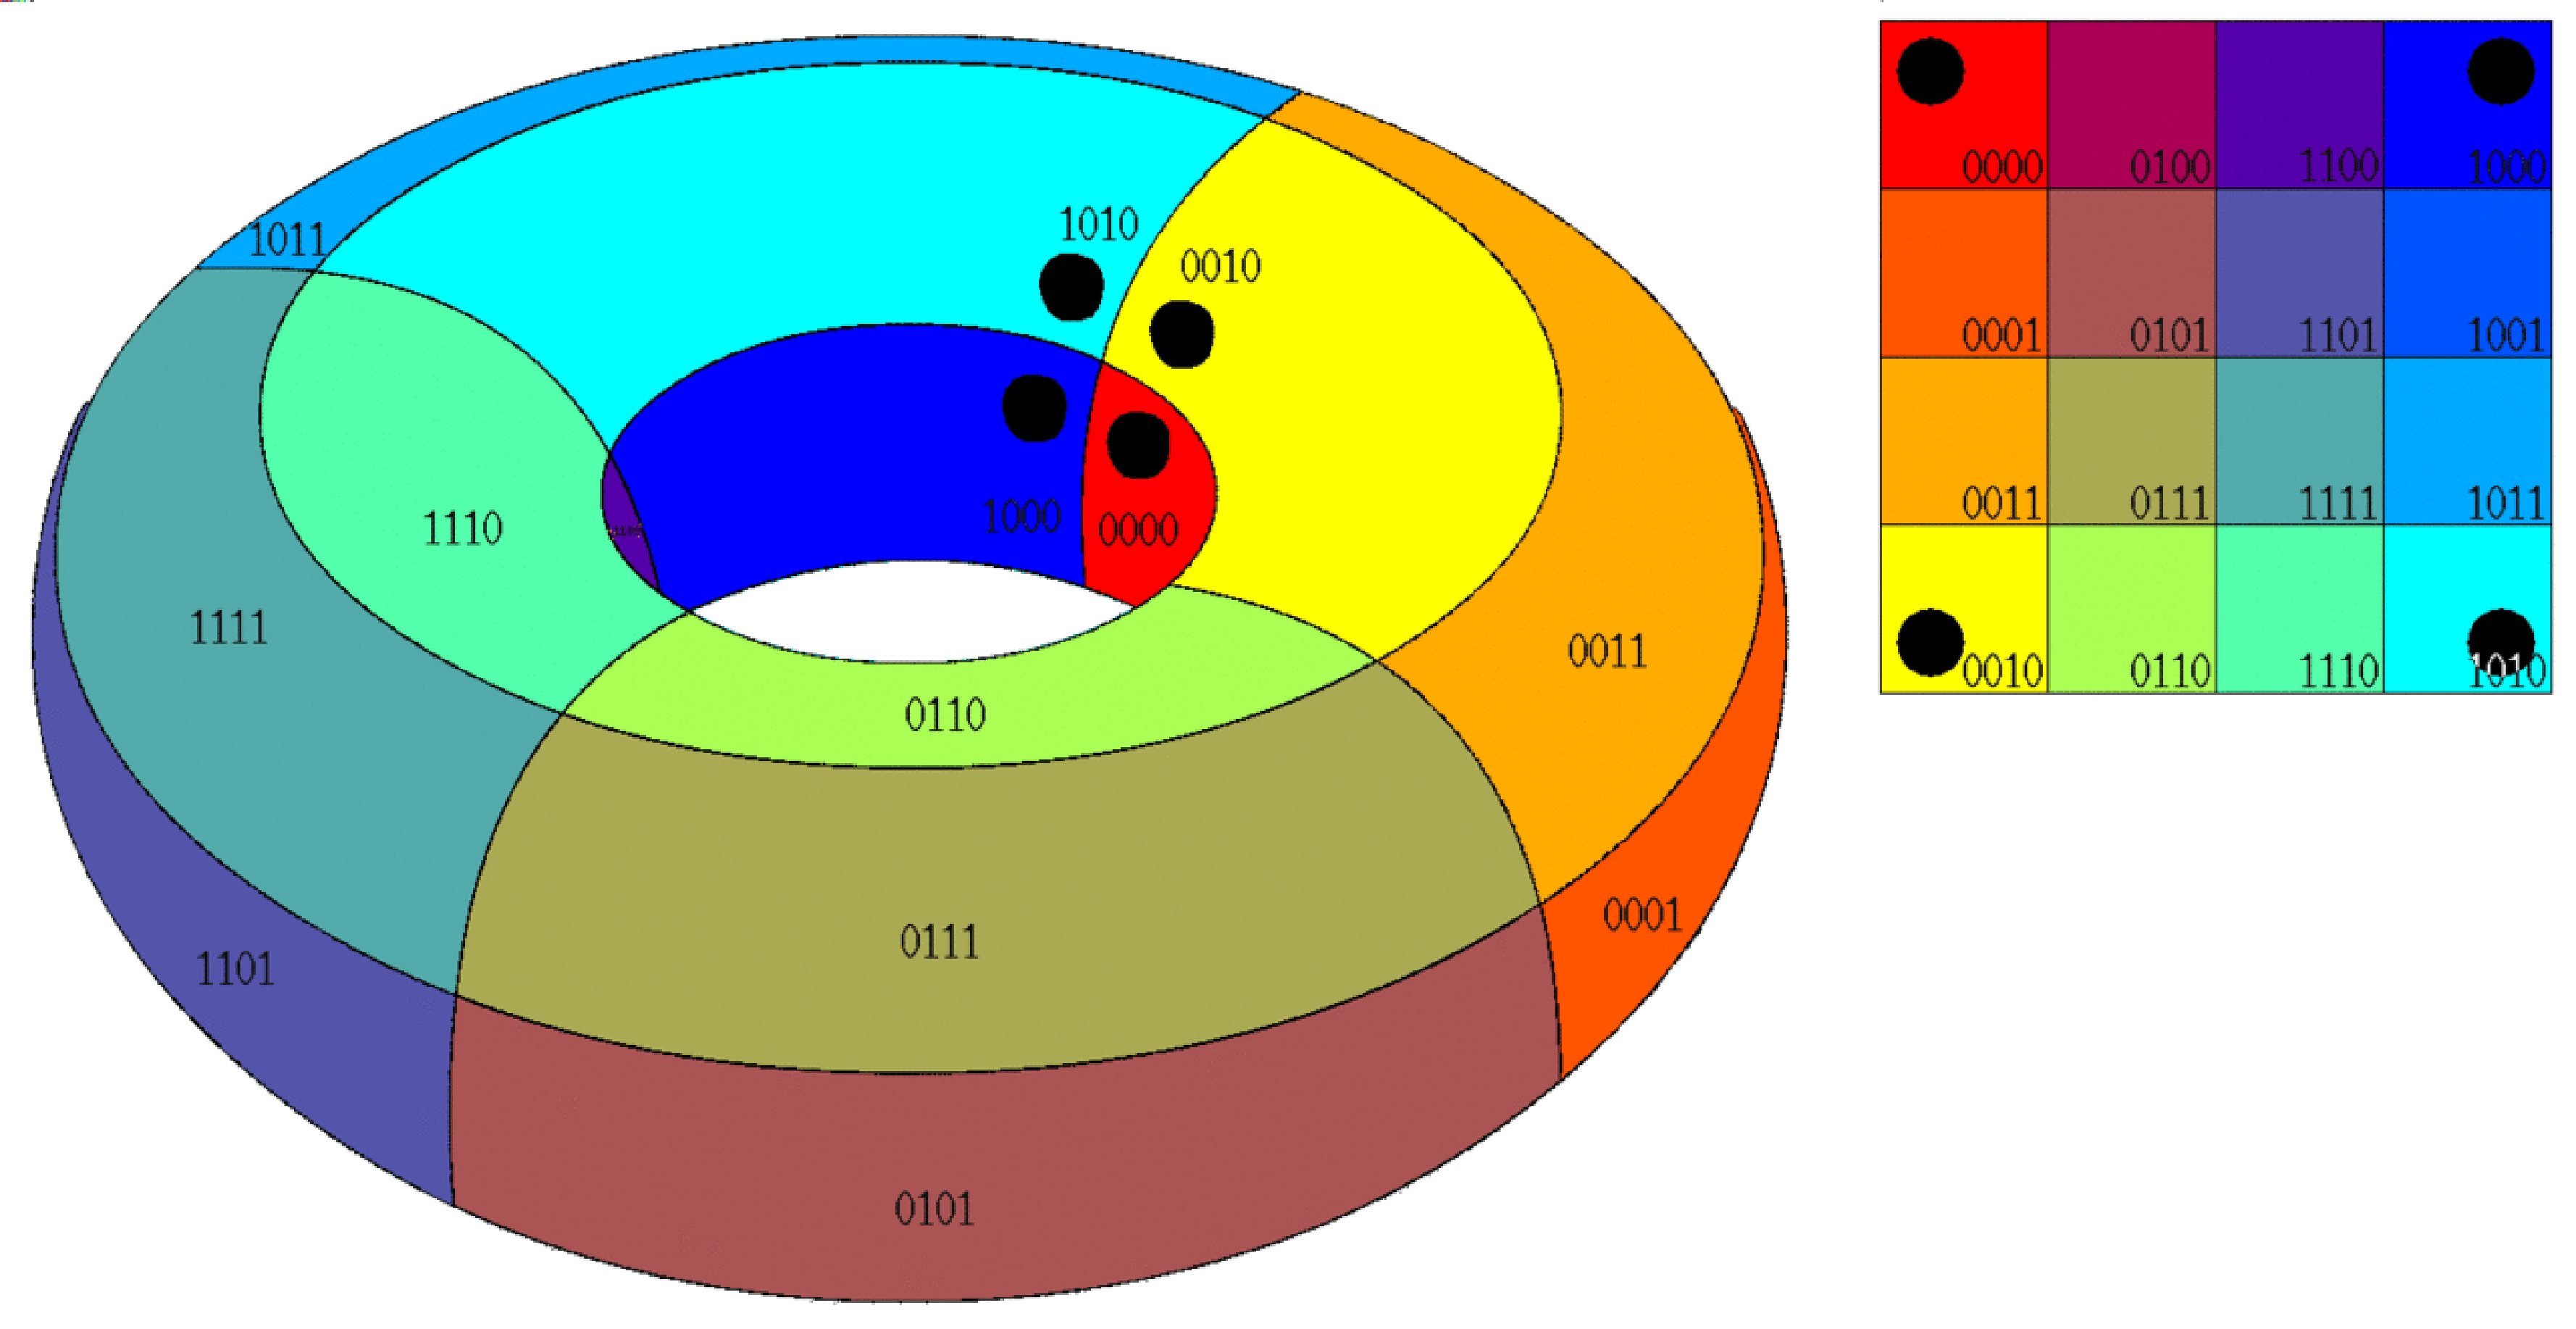
\includegraphics[width=\columnwidth]{Figures/torus.png}

    Na pocetku se upise u svako polje odgovarajuca vrednost funkcije.
    Ako se dve jedinice nalaze jedna pored druge to znaci da se one mogu 
    grupisati, jer se razlikuju samo na jednom mestu.
    Slicno i ako imamo cetiri jedinice koje formiraju provougaonik
    Pravila zaokruzivanja:
    \begin{itemize}
        \itemsep0em
        \item Zaokruzuju se samo jedinice.
        \item Svaka jedinica mora da bude zaokruzena bar jednom.
        \item Mogu se zaokruzivati iskljucivo grupo od po $2^k$ polja 
              pravougaonog oblika.
        \item Uvek se zaokruzuju sto vece grupe, cak i ako se tom prilikom 
              neke jedinice ponovo zaokruzuju.
        \item Nakon sto se sve jednice zaokruze, treba proveriti da li je neko 
              od zaokruzivanja postalo suvisno, jer scako njegovo polje 
              pripada i nekom drugom zaokruzivanju.
    \end{itemize}

    Svakom od dobijenih zaokruzivanja odgovara jedna elementarna konjukcija
    koja sadrzi upravo one literale koju su zajednici za sva polja koja 
    obuhvata to zaokruzivanje.

    \subsection{Metod Kvin-Meklaskog}
    
    \section{Logicka Kola}
    
    \emph{Logicko kolo} (eng. \emph{logic circuit}) je uredjaj koji 
    implementira neki skup logickih funkcija u datoj tehnologiji.

    \subsection{Vrednost visoke impedense}
    
    Nekada je moguce da izlaz logickog nema nikakvu vrednost, tj.\ da mu
    izlazna vrednost nije ni 0 ni 1. Tu vrednost nazivamo 
    \emph{vrednost visoke impedense} i obelezavamo je sa $\mathbf{Z}$. Ukoliko
    neki izraz ima vrednost $\mathbf{Z}$, tada taj izraz ne uticne na vrednost 
    ulazna na koji je povezan.

    \subsection{Logicke Kapije}

    \emph{Logicke kapije} ili \emph{gejtovi} su uredjaju koji implementiraju 
    logicke veznika iz izabranog skupa.

    \begin{tabular}{*{3}{c}}
        Naziv kola & Sematska oznaka \\
        \midrule
        buffer  & 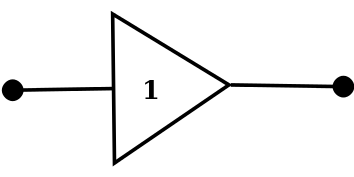
\includegraphics[width=30px]{Figures/buffer.png} \\
        NOT  & 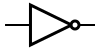
\includegraphics[width=30px]{Figures/not.png} \\
        AND  & 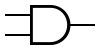
\includegraphics[width=30px]{Figures/and.png} \\
        OR   & 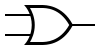
\includegraphics[width=30px]{Figures/or.png} \\
        NAND & 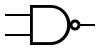
\includegraphics[width=30px]{Figures/nand.png} \\
        NOR  & 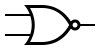
\includegraphics[width=30px]{Figures/nor.png} \\
        XOR  & 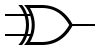
\includegraphics[width=30px]{Figures/xor.png} \\
        XNOR & 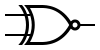
\includegraphics[width=30px]{Figures/xnor.png} \\
    \end{tabular}

    \subsection{Implementacija Logickih Kapija u Savremenim Racunarima}

    Savremeni racunari su zasnivani na jednoj posebnoj vrsti unipolarnih
    tranzistora --- \emph{MOS tranzistori} 
    (eng. \emph{Metal-Oxide-Semiconductor}).
    MOS predstavlja poluprovodnicku komponentu koja ima tri prikljucka:
    \emph{sors} (eng. \emph{source}), \emph{drejn} (eng \emph{drain}), i 
    \emph{gejt} (eng. \emph{gate}).
    MOS tranzistor funkcionise kao prekidac --- struja moze da protice od 
    sorsa ka drajnu po uslovom da se odgovarajuci napon dovede na gejt.
    Kroz gejt ne protice struja vec on stvara elektricno polje kroz koje
    ce struja da tece.
    Postoje dva tipa MOS tranzistora: NMOS i PMOS tranzistor.

    Kod NMOS tranzistora sopr mora biti prikljucen na negativan, a drejn na 
    pozitivan napon.
    Da bi doslo do provodjenja struje, potrebno je na gejt dovesti dovoljno 
    veliki pozitivan napon.
    Ukoliko je napon u zoni logicke nule, tada je tranzistor u potpunosti 
    zatvoren i ne provodi struju od sorsa ka drejnu, dok kada je u zoni 
    logicke jedinice od provodi struju.

    Kod PMOS tranzistora sors se prikljucuje na pozitivan, a drajn na negativan
    napon. 
    Da bi doslo do provodjenja struje, potrebno je na gejt dovesti negativan 
    napon.
    Ukoliko je napon u zoni logicke jedinice, tada je tranzistor u zatvoren i
    ne provodi struju, dok kada je u zoni logicke nule on provodi struju.

    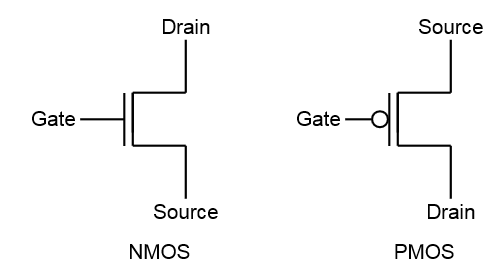
\includegraphics[width=0.8\columnwidth]{Figures/mos.png}

    Ako se u izradi logickig kola koriste i NMOS i PMOS tranzistori, tada
    govorimo o CMOS tehnologiji (eng. \emph{Complementary MOS}).

    \subsubsection{NOT kolo}

    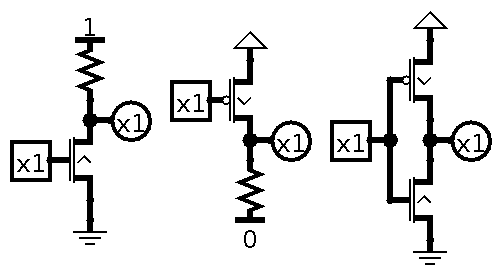
\includegraphics[width=0.7\columnwidth]{Figures/mos_not.png}

    \subsubsection{NAND i AND kolo}

    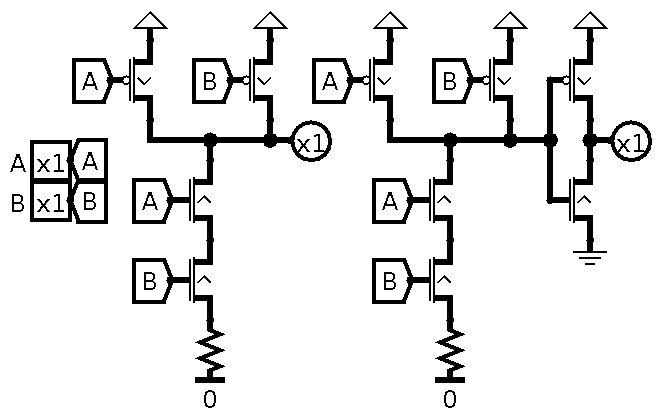
\includegraphics[width=0.8\columnwidth]{Figures/mos_nand_and.png}

    \subsubsection{NOR i OR kolo}

    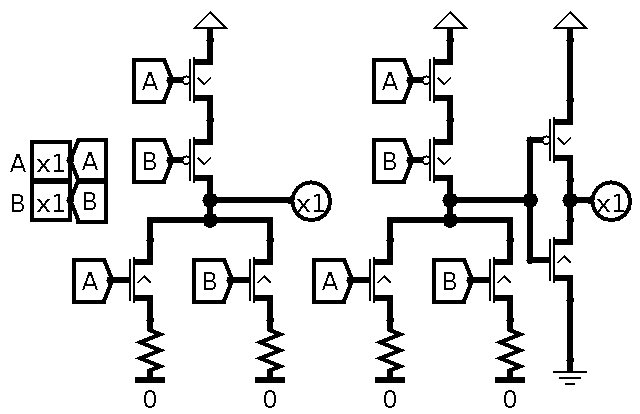
\includegraphics[width=0.8\columnwidth]{Figures/mos_nor_or.png}

    \subsubsection{XOR kolo}

    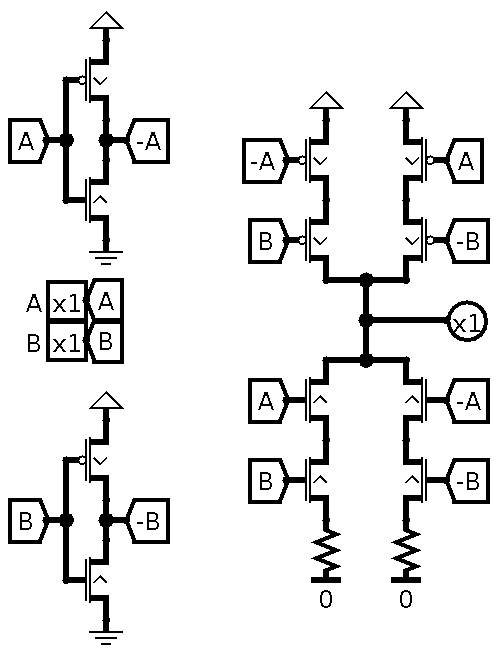
\includegraphics[width=0.7\columnwidth]{Figures/mos_xor.png}

    \subsubsection{Buffer}

    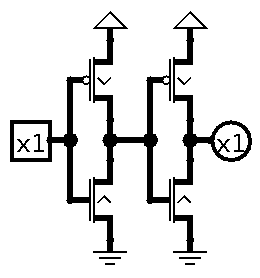
\includegraphics[width=0.4\columnwidth]{Figures/mos_buffer.png}

    \subsubsection{Propusni Tranzistori i Prenosne Kapije}

    \emph{Propusni tranzistori} kontrolisu propustanje nekog signala od jedne 
    tacke kola ka drugoj u zavisnost od vrednosti nekog drugog signala.

    \emph{Propusna kapija} CMOS varijanta propusnih tranzistora.

    \subsection{Baferi sa Tri Stanja}

    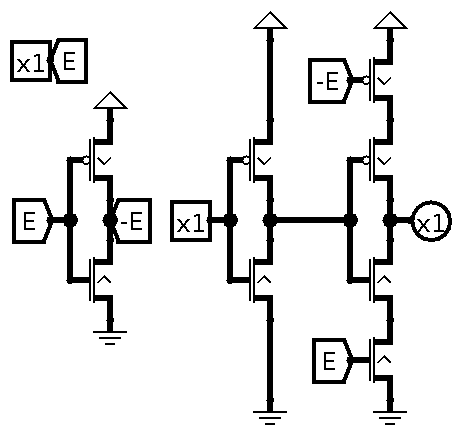
\includegraphics[width=0.7\columnwidth]{Figures/mos_tristate_buffer.png}
    
    \section{Kombinatorna Kola}

    \section{Sekvencijalna Kola}
    
    

\end{multicols}

\end{document}
